%
% $RCSfile: human_thinking.tex,v $
%
% Copyright (c) 2004. Christian Heller. All rights reserved.
%
% No copying, altering, distribution or any other actions concerning this
% document, except after explicit permission by the author!
% At some later point in time, this document is planned to be put under
% the GNU FDL license. For now, _everything_ is _restricted_ by the author.
%
% http://www.cybop.net
% - Cybernetics Oriented Programming -
%
% http://www.resmedicinae.org
% - Information in Medicine -
%
% @author Christian Heller <christian.heller@tuxtax.de>
%

\subsection{Human Thinking}
\label{human_thinking_heading}

The new classification is based on the idea of categorizing software patterns
after the principles of \emph{Human Thinking}, that is concepts of the logical
\emph{Mind}, as opposed to \emph{Artificial Neural Networks} (ANN) that want to
imitate the functioning of the physical \emph{Brain}.

The corresponding concepts were first introduced in \cite{heller2004}. After an
investigation of the fundamentals of human thinking, that is how human beings
understand their surrounding real world by abstracting it in \emph{Models}, that
paper concludes that there were three basic activities of abstraction:

\begin{enumerate}
    \item Discrimination
    \item Categorization
    \item Composition
\end{enumerate}

By discriminating their environment, humans are able to share it into discrete
\emph{Items}. Items with similar properties can be classified into a common super
\emph{Category}. Any abstract model of the universe is just an illusion, being
made up of yet smaller models, and nobody knows where this hierarchy really stops,
towards microcosm as well as towards macrocosm. Therefore, the third and last
kind of abstraction, namely composition, lets humans perceive the items in their
environment as \emph{Compound} of smaller items.

\begin{figure}[ht]
    \begin{center}
        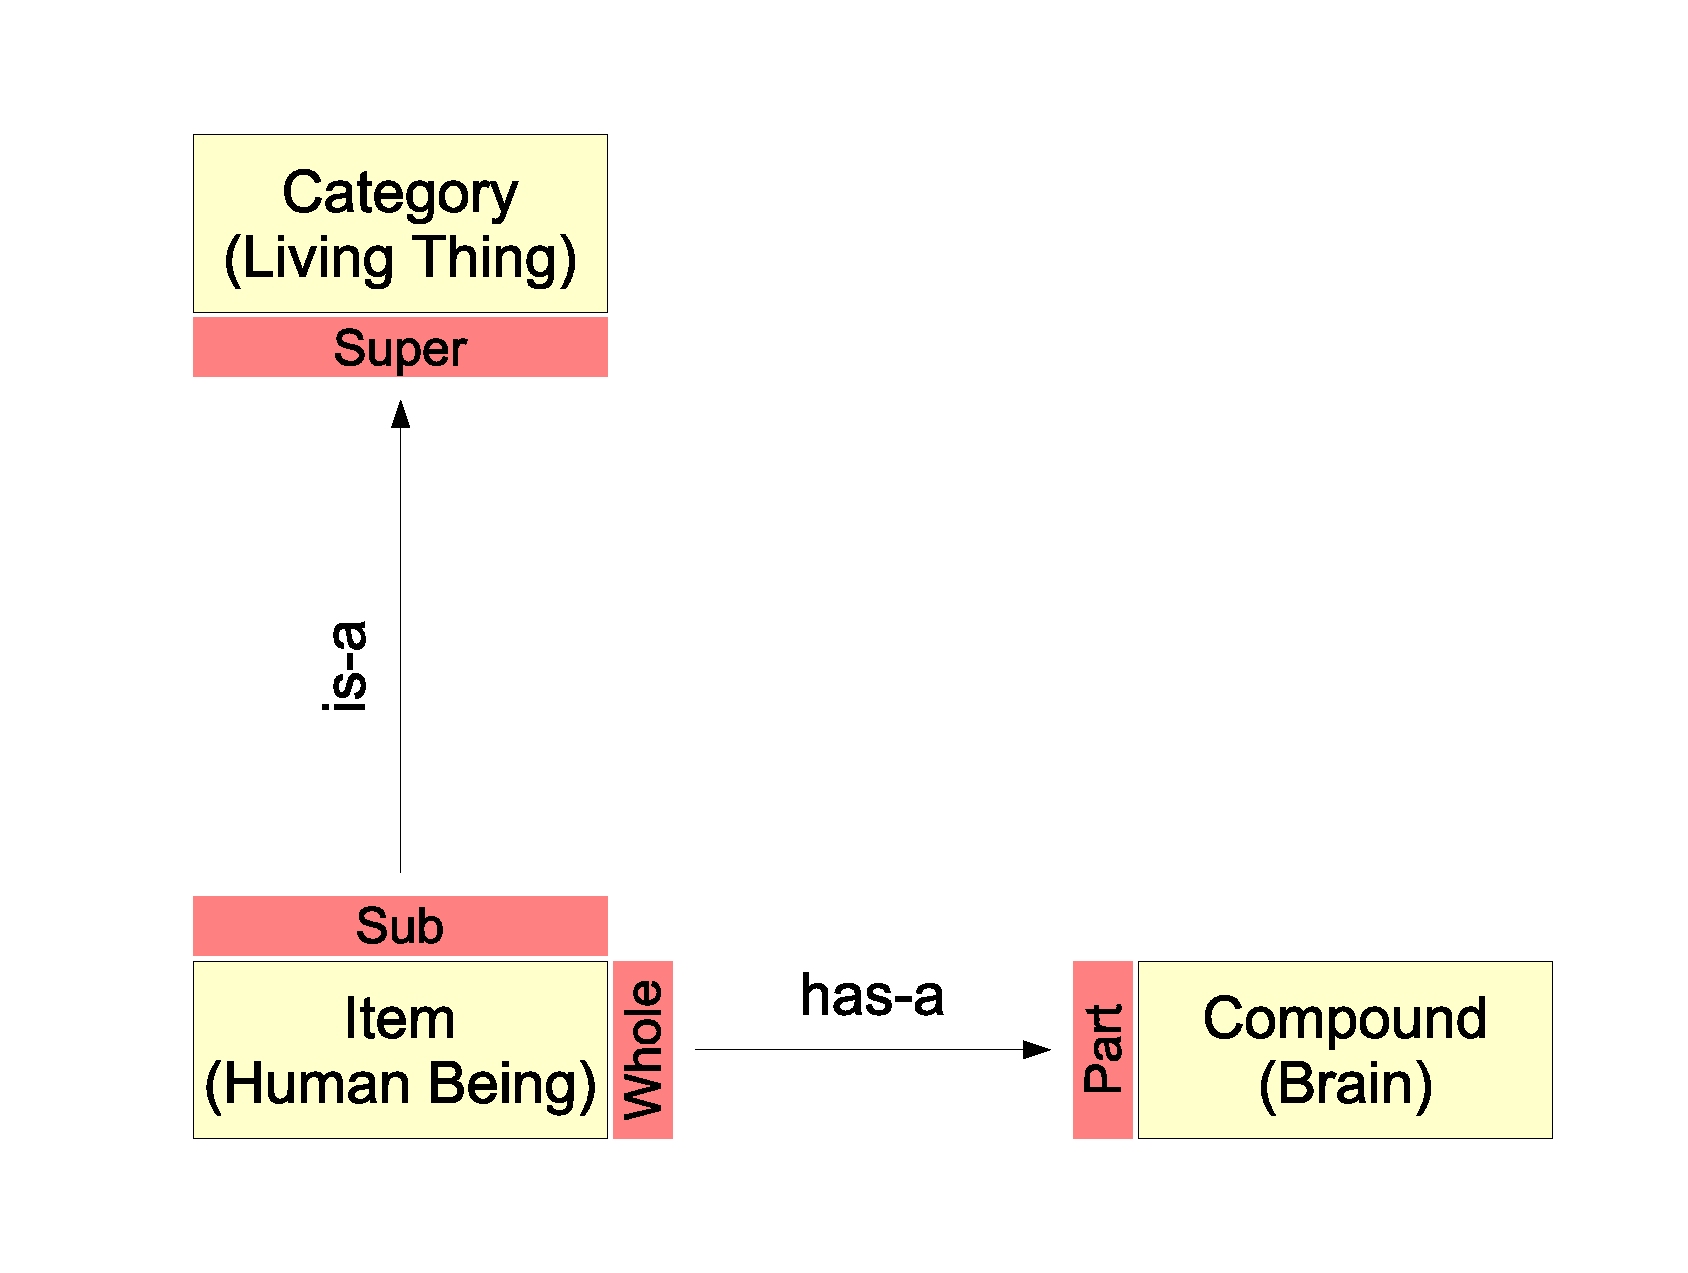
\includegraphics[scale=0.3]{vector/abstraction.eps}
        \caption{Abstractions of Human Thinking \cite{heller2004}}
        \label{abstraction_figure}
    \end{center}
\end{figure}

The latter two activities of abstraction -- categorization and composition --
are based on special \emph{Associations} (figure \ref{abstraction_figure}),
between a \emph{Super-} and a \emph{Sub} model and between a \emph{Whole-} and
a \emph{Part} model, respectively.
